\documentclass{beamer}
\usepackage[utf8]{inputenc}
\usepackage{hyperref}

\usepackage{tikz}

\usepackage{latexsym,xcolor,multicol,booktabs,calligra}
\usepackage{amsmath,amssymb,BOONDOX-cal,bm}
\usepackage{graphicx,pstricks,stackengine}
\usepackage{libertinus}
\usepackage{amssymb}
\usepackage{pgfplots}
\usepackage{tikz}
\usepackage{xcolor}
\usetikzlibrary{positioning,arrows.meta,shapes.geometric}

\usepackage{etoolbox}
\makeatletter
\newcommand{\noframenumbering}{%
  \beamer@noframenumberingtrue%
}
\makeatother

\usepackage[T1]{fontenc}

\usepackage{hyperref}
\hypersetup{
    colorlinks=true,
    linkcolor=blue,
    urlcolor=blue,
    citecolor=blue
}

\title{Macroeconometrics\\
9 - Bayesian Estimation: Foundations and Applications to VARs}
\author{Camille Souffron\\
Ecole Normale Supérieure \& Paris School of Economics\\
\textcolor{blue}{\href{mailto:camille.souffron@ens.psl.eu}{camille.souffron@ens.psl.eu}}}
\institute{\normalsize M2 EPOG JM}
\date{Fall 2026}

\usetheme{Singapore}

\def\cmd#1{\texttt{\color{red}\footnotesize $\backslash$#1}}
\def\env#1{\texttt{\color{RoyalBlue}\footnotesize #1}}

\newtheorem{thm}{Theorem}[theorem]
\setbeamertemplate{footline}[frame number]

\begin{document}

\begin{frame}
    \titlepage
    \begin{center}
        
\includegraphics[width=0.5\textwidth]{logos.png}
    \end{center}
\end{frame}

\addtocounter{framenumber}{-1}


%======================================================
\section{Why Bayesian?}
%======================================================

%======================================================
\begin{frame}{What We Have Been Doing So Far - and Its Limits}
%======================================================
\small

\textbf{All estimation so far was frequentist:}
\begin{itemize}
\footnotesize
  \item Parameters $\theta$ are \textbf{fixed but unknown} constants.
  \item We find the value of $\theta$ that best fits the data (OLS, MLE, GMM...).
  \item Uncertainty is expressed via \textbf{asymptotic} standard errors and confidence intervals
        ($\approx$ ``if we repeated the experiment infinitely often...'').
\end{itemize}

\pause
\medskip
\textbf{Problems in macro:}
\begin{itemize}
\footnotesize
  \item \textbf{Short time series:} $T = 40$-$150$ observations. Asymptotics are a \textit{bogus}.
  \item \textbf{Many parameters:} a VAR$(p)$ with $k$ variables has $k^2 p$ slope parameters $+ k(k+1)/2$ covariance parameters.
        With $T = 120$ quarterly observations (30y) and $k=8, p=4$: \textbf{264 parameters}!  $k=8, p=4$: OLS estimates \textbf{292 parameters} from 120 observations! Catastrophic over-fitting. IRFs and forecasts are \textbf{garbage}.
  \item \textbf{Structural breaks, regime changes:} time-varying parameters $\Rightarrow$ even fewer effective observations per regime.
  \item \textbf{We often know something} \textit{\textbf{before}} looking at the data (economic theory, stylized facts, previous studies). Frequentist methods do not use this.
\end{itemize}

\pause
\medskip
\textcolor{blue}{\textbf{Bayesian solution:}
\footnotesize
treat $\theta$ as a \textbf{random variable}. Express what we know \emph{before} seeing the data
as a \textbf{prior distribution}, update it with the data to get a \textbf{posterior distribution}}.


\end{frame}


%======================================================
\begin{frame}{Bayes' Theorem (The Core Idea)}
%======================================================
\small

\[
\underbrace{p(\theta \mid Y)}_{\textbf{posterior}}
\;\propto\;
\underbrace{p(Y \mid \theta)}_{\textbf{likelihood}}
\;\times\;
\underbrace{p(\theta)}_{\textbf{prior}}
\]

\medskip
\begin{itemize}
  \item $p(\theta)$: \textbf{prior} - what we believe about $\theta$ \emph{before} seeing data (theoretical knowledge, stylized facts, regularization, known empirics).
  \item $p(Y \mid \theta)$: \textbf{likelihood} - how probable is the observed data $Y$
        given parameter value $\theta$? (Same object as in \textbf{MLE}!)
  \item $p(\theta \mid Y)$: \textbf{posterior} - updated belief about $\theta$ \emph{after}
        seeing data $=$ our full inference object.
\end{itemize}

\pause
\medskip
\textbf{Conceptual shifts vs. frequentism:}
\begin{enumerate}
  \item Uncertainty about $\theta$ is \textbf{probabilistic} (not hypothetically repeated sampling).
  \item The posterior is a \textbf{distribution} over $\theta$ (not a point estimate $+$ SE).
  \item As $T \to \infty$, the prior is \textbf{washed out} by the data: posterior $\to$ MLE
        (Bernstein-von Mises theorem). \textbf{But with small $T$: the prior matters!}
\end{enumerate}

\end{frame}


%======================================================
\begin{frame}{Example: AR(1) with a Prior}
%======================================================
\small

\textbf{Model:} $y_t = \phi\, y_{t-1} + \varepsilon_t$, $\varepsilon_t \sim \mathcal{N}(0, \sigma^2)$.

\medskip
\textbf{OLS/MLE (frequentist):} $\hat\phi = \frac{Cov( y_t y_{t-1})}{Var(y_{t-1}^2)}$. No prior. With $T=30$ and a near-unit-root process (e.g.\ true $\phi = 0.99$), then $\hat\phi$ can be e.g.\ $1.02$ or $0.78$ by pure \textit{sampling variation.}

\medskip
\textbf{Bayesian:} place a prior $\phi \sim \mathcal{N}(1,\, \kappa^2)$ (``random walk is a reasonable benchmark'').

\medskip
The posterior mean is a \textbf{weighted average}:
\[
\mathbb{E}[\phi \mid Y] = \underbrace{\frac{T/\sigma^2}{T/\sigma^2 + 1/\kappa^2}}_{\text{weight on data}} \hat\phi_{\text{OLS}}
+ \underbrace{\frac{1/\kappa^2}{T/\sigma^2 + 1/\kappa^2}}_{\text{weight on prior}} \cdot 1
\]

\begin{itemize}
  \item Small $T$: prior dominates $\Rightarrow$ shrinks $\phi$ toward 1 (random walk).
  \item Large $T$: data dominates $\Rightarrow$ posterior $\approx$ OLS.
  \item \textbf{Shrinkage = regularization}: same spirit as ridge regression, but fully probabilistic.
\end{itemize}

\end{frame}


%======================================================
\begin{frame}{Prior, Likelihood, Posterior }
%======================================================
\begin{center}
  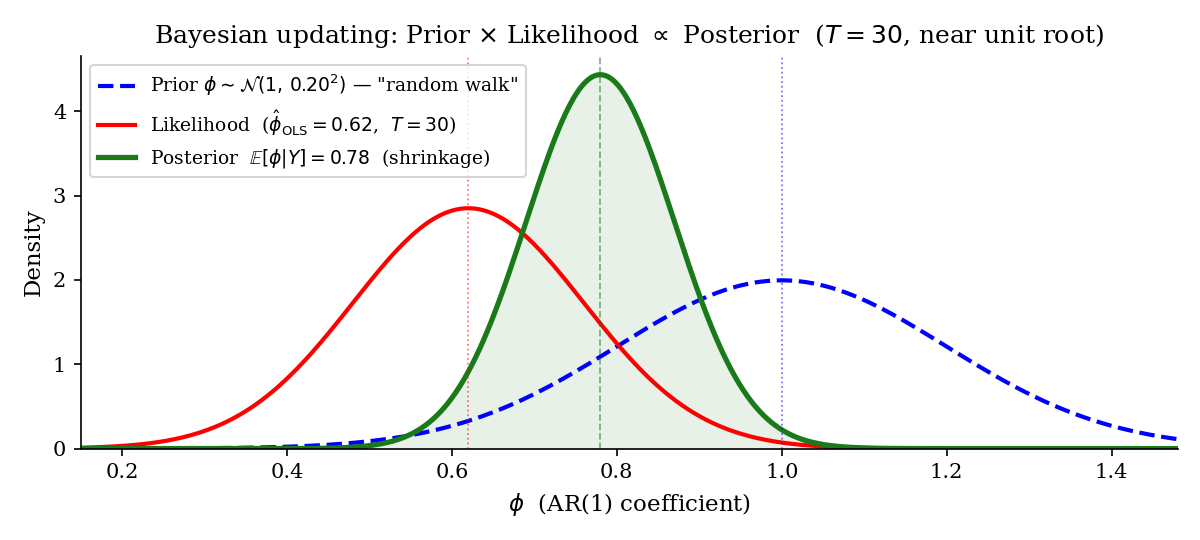
\includegraphics[width=0.90\textwidth]{image/prior_posterior_ar1.png}
\end{center}
\vspace{-0.3cm}
\footnotesize
\begin{itemize}
  \item OLS ($\hat\phi=0.62$, $T=30$): wide likelihood (can be even flatter) - large sampling noise.
        The prior $\mathcal{N}(1,0.20^2)$ pulls the posterior toward $1$ while allowing for large variance - \textbf{shrinkage}.
  \item The posterior is \textbf{narrower} than either component: combining information reduces uncertainty.
  \item \textbf{Posterior credible interval} $\neq$ frequentist CI: ``$\phi$ lies here with probability 90\%'' (direct probability statement, not a repeated-sampling statement).
\end{itemize}

\end{frame}


%======================================================
\begin{frame}{What is the Prior? Is it Subjective?}
%======================================================
\small

\textbf{A prior can come from:}
\begin{enumerate}
  \item \textbf{Economic theory:} e.g.\ price homogeneity imposes constraints on long-run elasticities. Or stationarity of consumption/income ratio $\Rightarrow$ cointegration $\Rightarrow$ prior on ECM coefficient.
  \item \textbf{Stylized facts from the literature:} e.g. monetary policy multipliers are small in the first quarter (lags in transmission). Prior: impact IRF $\sim \mathcal{N}(0, 0.1^2)$.
  \item \textbf{Regularization / parsimony:} no strong theoretical view / empirical benchmark? Use a prior that \textbf{shrinks toward a simple benchmark} (random walk, zero cross-equation spillovers...).
  \item \textbf{Non-informative / diffuse prior:} $p(\theta) \propto 1$ (``let the data speak entirely.''). Posterior then $\approx$ likelihood. Useful for comparison.
\end{enumerate}

\pause
\medskip
\textcolor{red}{\textbf{Objectivity?}}
\medskip

The prior is a \textbf{modelling choice like any other} (e.g.\ choosing lag length, functional form, identifying restrictions). Difference: it is \textbf{explicit and transparent}. Frequentist methods
also embed implicit regularization (ridge, LASSO, lag selection rules) but Bayesian methods make it visible.


\end{frame}


%======================================================
\begin{frame}{Posterior Summaries - What Do We Report?}
%======================================================
\small

The posterior $p(\theta \mid Y)$ is a full distribution. We summarize it:

\medskip
\begin{tabular}{lll}
\toprule
\textbf{Summary} & \textbf{Formula} & \textbf{Frequentist analogue} \\
\midrule
Posterior mean & $\hat\theta = \mathbb{E}[\theta \mid Y]$ & Point estimate \\
Posterior mode & $\arg\max_\theta p(\theta \mid Y)$ & MAP / penalized MLE \\
Posterior std & $\sqrt{\text{Var}(\theta \mid Y)}$ & Standard error \\
Credible interval & $P(a \le \theta \le b \mid Y) = 1-\alpha$ & Confidence interval \\
\bottomrule
\end{tabular}

\medskip
\textbf{Posterior predictive distribution:}
\[
p(y_{T+h} \mid Y) = \int p(y_{T+h} \mid \theta)\, p(\theta \mid Y)\, d\theta
\]
Forecasts that \textbf{integrate over parameter uncertainty} - automatically wider than plug-in forecasts.
Crucial in macro where $\theta$ is poorly identified with short samples.

\smallskip 
\textbf{Model comparison via marginal likelihood:}
\[
p(Y \mid \mathcal{M}) = \int p(Y \mid \theta, \mathcal{M})\, p(\theta \mid \mathcal{M})\, d\theta
\Rightarrow \text{Bayes Factor} = \frac{p(Y \mid \mathcal{M}_1)}{p(Y \mid \mathcal{M}_2)}
\]
Automatically penalizes over-parameterization (\textit{Occam's razor} built in).

\end{frame}


%======================================================
\section{Bayesian Computation}
%======================================================

%======================================================
\begin{frame}{The Computational Problem}
%======================================================
\footnotesize

\textbf{In simple models:} posterior has an analytical form.
\begin{itemize}
  \item Normal likelihood + Normal prior on $\mu$ $\Rightarrow$ Normal posterior (conjugate pair).
  \item Normal-Wishart prior on $(B, \Sigma)$ in a VAR $\Rightarrow$ Normal-Wishart posterior.
\end{itemize}

\medskip
\textbf{In general:} the posterior is a high-dimensional integral with no closed form.
\[
p(\theta \mid Y) = \frac{p(Y \mid \theta)\, p(\theta)}{\int p(Y \mid \theta)\, p(\theta)\, d\theta}
\]
The denominator (\textbf{marginal likelihood / normalizing constant}) is \emph{intractable} for most models.

\pause
\medskip
\textbf{Solution: Markov Chain Monte Carlo (MCMC).}

Instead of computing the posterior analytically, \textbf{draw samples} $\{\theta^{(s)}\}_{s=1}^S$ from
$p(\theta \mid Y)$ and use sample averages as estimators:
\[
\mathbb{E}[g(\theta) \mid Y] \approx \frac{1}{S}\sum_{s=1}^S g(\theta^{(s)})
\]
Works for \emph{any} posterior - even if the likelihood is non-Gaussian or the model is nonlinear.

\end{frame}


%======================================================
\begin{frame}{MCMC: Gibbs Sampler (the workhorse in macro)}
%======================================================
\footnotesize

\textbf{Idea:} if sampling from the \emph{joint} posterior $p(\theta_1, \theta_2, \dots \mid Y)$ is hard,
sample iteratively from \textbf{full conditionals} $p(\theta_j \mid \theta_{-j}, Y)$ - which are often tractable.

\medskip
\textbf{Algorithm:}
\begin{enumerate}
  \item Initialize $\theta^{(0)} = (\theta_1^{(0)}, \theta_2^{(0)}, \dots)$.
  \item For $s = 1, 2, \dots, S$:
  \begin{enumerate}
  \footnotesize
    \item Draw $\theta_1^{(s)} \sim p(\theta_1 \mid \theta_2^{(s-1)}, \theta_3^{(s-1)}, \dots, Y)$
    \item Draw $\theta_2^{(s)} \sim p(\theta_2 \mid \theta_1^{(s)},   \theta_3^{(s-1)}, \dots, Y)$
    \item \dots
  \end{enumerate}
  \item Discard first $S_0$ draws (\textbf{burn-in}); use $\{\theta^{(s)}\}_{s=S_0+1}^S$ for inference.
\end{enumerate}

\medskip
\textbf{Why it works:} the chain $\{\theta^{(s)}\}$ has $p(\theta \mid Y)$ as its \textbf{stationary distribution}
(detailed balance condition). After convergence, draws are (approximately) i.i.d.\ from the posterior. \textbf{In practice:}
\begin{itemize}
  \item Check \textbf{convergence}: trace plots, Gelman-Rubin $\hat R < 1.1$ across multiple chains.
  \item \textbf{Autocorrelation} in the chain reduces effective sample size $\Rightarrow$ run long chains.
  \item \textbf{Metropolis-Hastings} step: if a full conditional has no closed form, use a proposal $+$ acceptance/rejection step (MH within Gibbs).
\end{itemize}

\end{frame}


%======================================================
\begin{frame}{MCMC: Convergence in Practice}
%======================================================
\begin{center}
  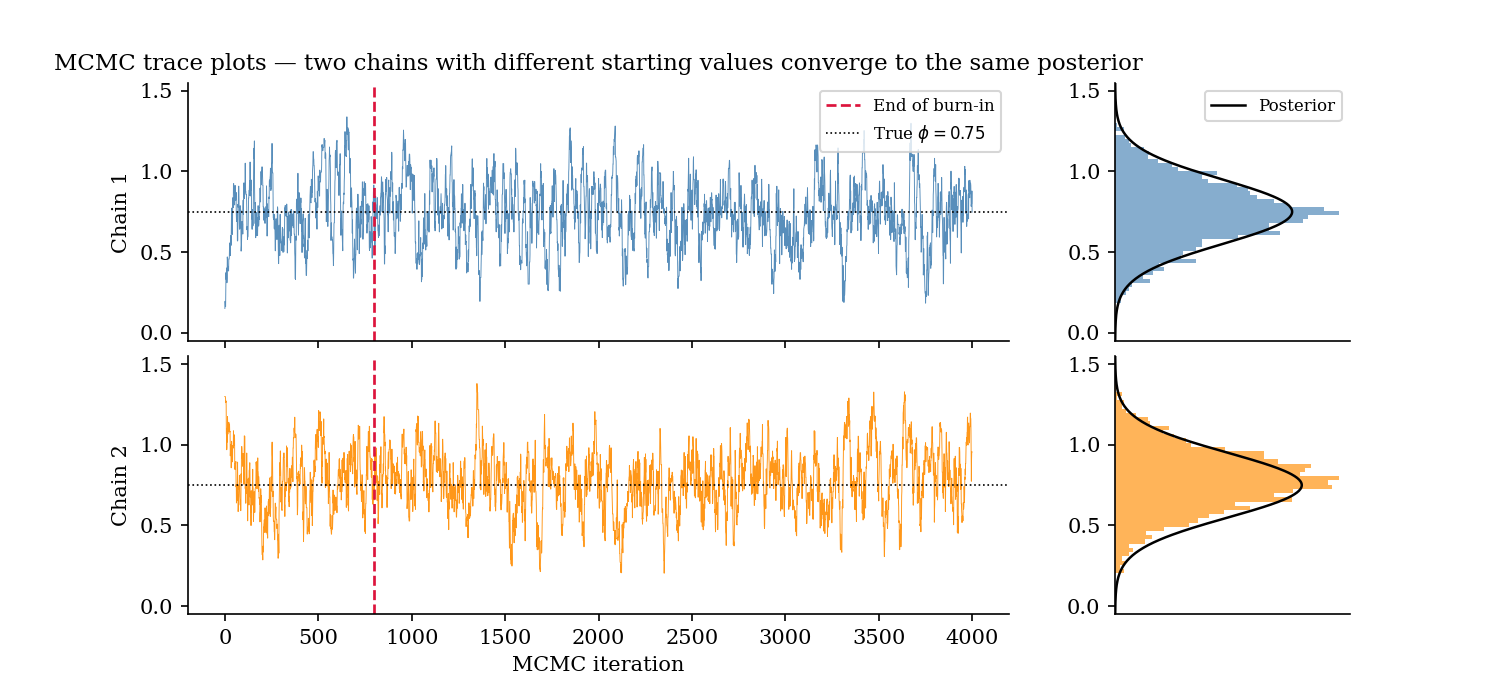
\includegraphics[width=0.94\textwidth]{image/mcmc_trace.png}
\end{center}
\vspace{-0.3cm}
\footnotesize\centering
Two chains starting at $\phi^{(0)}=0.15$ and $\phi^{(0)}=1.30$. After the burn-in (red dashed line) both chains mix around the true value $\phi=0.75$.\\

Right panels: marginal histogram of post-burn-in draws vs.\ analytical posterior density - good agreement confirms convergence.
\end{frame}


%======================================================
\begin{frame}{MCMC: Metropolis-Hastings and Modern Samplers}
%======================================================
\footnotesize

\textbf{Metropolis-Hastings (MH):} when $p(\theta \mid Y)$ has no closed form.
\begin{enumerate}
  \item At state $\theta^{(s-1)}$, propose $\theta^* \sim q(\theta^* \mid \theta^{(s-1)})$ (e.g.\ Gaussian random walk).
  \item Accept with probability:
  \[
    \alpha = \min\!\left(1,\; \frac{p(\theta^* \mid Y)\, q(\theta^{(s-1)} \mid \theta^*)}{p(\theta^{(s-1)} \mid Y)\, q(\theta^* \mid \theta^{(s-1)})}\right)
  \]
  \item If accepted: $\theta^{(s)} = \theta^*$. Else: $\theta^{(s)} = \theta^{(s-1)}$.
\end{enumerate}

\medskip
\textbf{Modern alternatives} (avoid slow random-walk exploration):
\begin{itemize}
  \item \textbf{HMC (Hamiltonian Monte Carlo):} uses gradient of $\log p(\theta \mid Y)$ to make
        ``directed'' proposals. Much lower autocorrelation. Implemented in \texttt{Stan}.
  \item \textbf{NUTS (No-U-Turn Sampler):} adaptive HMC. Default in \texttt{Stan}, \texttt{PyMC}.
  \item \textbf{Variational Bayes:} approximate the posterior by a tractable family (e.g.\ Gaussian)
        minimizing KL divergence. \textbf{Very fast} but approximate. Useful for large models.
\end{itemize}

\medskip
\textbf{Conjugate priors shortcut:} when prior and likelihood are \textbf{conjugate}, the posterior is in
the same family as the prior $\Rightarrow$ \textbf{no MCMC needed}, analytical update.
(Normal-Wishart for VARs: see next section.)

\end{frame}


%======================================================
\section{Bayesian VARs - Priors}
%======================================================

%======================================================
\begin{frame}{Why Bayesian VARs?}
%======================================================
\small

\textbf{Bayesian solution} to avoid catastrophic over-fitting (sometimes even more parameters to estimate than available observations!): place a prior that \textbf{shrinks} the VAR toward a parsimonious benchmark (random walk, zero cross-variable lags).
\medskip

If the signal is strong enough, the data can \textbf{override} the prior.
\medskip

$\Rightarrow$ \textbf{This is exactly regularization, but done in a probabilistically coherent way.}

\end{frame}


%======================================================
\begin{frame}{The General Bayesian VAR Setup}
%======================================================
\footnotesize

\textbf{VAR$(p)$ in matrix form:}
\[
Y = X B + E,
\qquad
E \sim \mathcal{MN}(0,\, T,\, \Sigma)
\]
\begin{itemize}
  \item $Y$: $T \times k$ matrix of observations.
  \item $X$: $T \times (kp+1)$ matrix of regressors (lags $+$ constant).
  \item $B$: $(kp+1) \times k$ coefficient matrix. \textbf{This is what we want to estimate.}
  \item $\Sigma$: $k \times k$ error covariance matrix.
\end{itemize}

\medskip
\textbf{Prior:} $p(B, \Sigma)$ encodes what we know before data.

\textbf{Likelihood:} $p(Y \mid B, \Sigma)$ - Gaussian, same as in OLS/MLE.

\textbf{Posterior:} $p(B, \Sigma \mid Y) \propto p(Y \mid B, \Sigma)\, p(B, \Sigma)$.

\medskip
\textbf{Posterior inference:}
\begin{itemize}
  \item Point estimates: posterior mean of $B$ and $\Sigma$.
  \item Forecasts: draw $(B^{(s)}, \Sigma^{(s)})$ from posterior, simulate forward $\Rightarrow$ \textbf{posterior predictive distribution}.
  \item IRFs: for each draw $B^{(s)}$, compute IRF$^{(s)}$ $\Rightarrow$ \textbf{credible bands} across draws.
\end{itemize}

\end{frame}


%======================================================
\begin{frame}{Prior 1 - Minnesota Prior (Litterman, 1979)}
%======================================================
\scriptsize

\textbf{The most widely used prior in macro VARs.} Introduced by Litterman (1979) at the Minneapolis Fed.

\medskip
\textbf{Benchmark belief:} ``each variable follows a \textbf{random walk}.
Cross-variable lags are probably small (or zero).''

\medskip
\textbf{Prior on coefficient $B_{\ell,ij}$ (lag $\ell$, effect of variable $j$ on variable $i$):}
\[
B_{\ell,ij} \sim \mathcal{N}\!\left(\mu_{\ell,ij},\; v_{\ell,ij}^2\right)
\]
\[
\mu_{\ell,ij} = \begin{cases} 1 & \text{if } i=j,\; \ell=1 \quad\text{(own first lag = random walk)} \\ 0 & \text{otherwise} \end{cases}
\]
\[
v_{\ell,ij}^2 = \begin{cases}
\left(\dfrac{\lambda_1}{\ell^{\lambda_3}}\right)^2 & \text{if } i=j \quad\text{(own lags, tighter at higher } \ell) \\[8pt]
\left(\dfrac{\lambda_1 \lambda_2}{\ell^{\lambda_3}} \cdot \dfrac{\sigma_i}{\sigma_j}\right)^2 & \text{if } i\neq j \quad\text{(cross-variable lags)} \\
\end{cases}
\]

\begin{itemize}
  \item $\lambda_1$: \textbf{overall tightness} ($\lambda_1 \to 0$: prior dominates, $\lambda_1 \to \infty$: OLS).
  \item $\lambda_2$: \textbf{cross-variable tightness} (typically $\lambda_2 < 1$: cross-lags shrunk harder than own).
  \item $\lambda_3$: \textbf{lag decay} (higher $\Rightarrow$ higher lags shrunk more aggressively, typically 1 or 2).
  \item $\sigma_i/\sigma_j$: scale correction so prior is scale-invariant.
\end{itemize}

\end{frame}


%======================================================
\begin{frame}{Minnesota Prior - Intuition and Implementation}
%======================================================
\footnotesize

\textbf{Why random walk as the benchmark?}
\begin{itemize}
  \item Many macro series (GDP, prices, interest rates) behave approximately as random walks or near-unit-root processes ($\phi$ close to $1$).
  \item A random walk is the ``most agnostic'' prior for persistent series: no mean reversion, no trend, just accumulation of the past.
  \item \textbf{If the data strongly supports }mean reversion or cross-variable dynamics, the posterior \textbf{will deviate from the prior} accordingly.
\end{itemize}

\medskip
\textbf{What does the prior actually do?}
\begin{itemize}
  \item Own first lag $\approx 1$: persistence is the default.
  \item Higher own lags $\approx 0$: past dynamics decay (the first lag already contains most information).
  \item Cross-variable lags $\approx 0$: VAR shrinks toward $k$ independent random walks.
        Only variables with true predictive power on themselves or on others survive.
\end{itemize}

\medskip
\textbf{Estimation:} the original Minnesota prior treats $\Sigma$ as \textbf{fixed} (diagonal, set from univariate regressions). Posterior on $B$ is then \textbf{analytically available} (Normal). \textbf{Very fast.}

\medskip
Standard choice for VARs. Excellent out-of-sample forecasting performance
(cf.\ Banbura, Giannone \& Reichlin, 2010, for large BVARs $(k = 20-100)$).

\end{frame}


%======================================================
\begin{frame}{Minnesota Prior - OLS vs.\ BVAR: IRF Comparison}
%======================================================
\begin{center}
  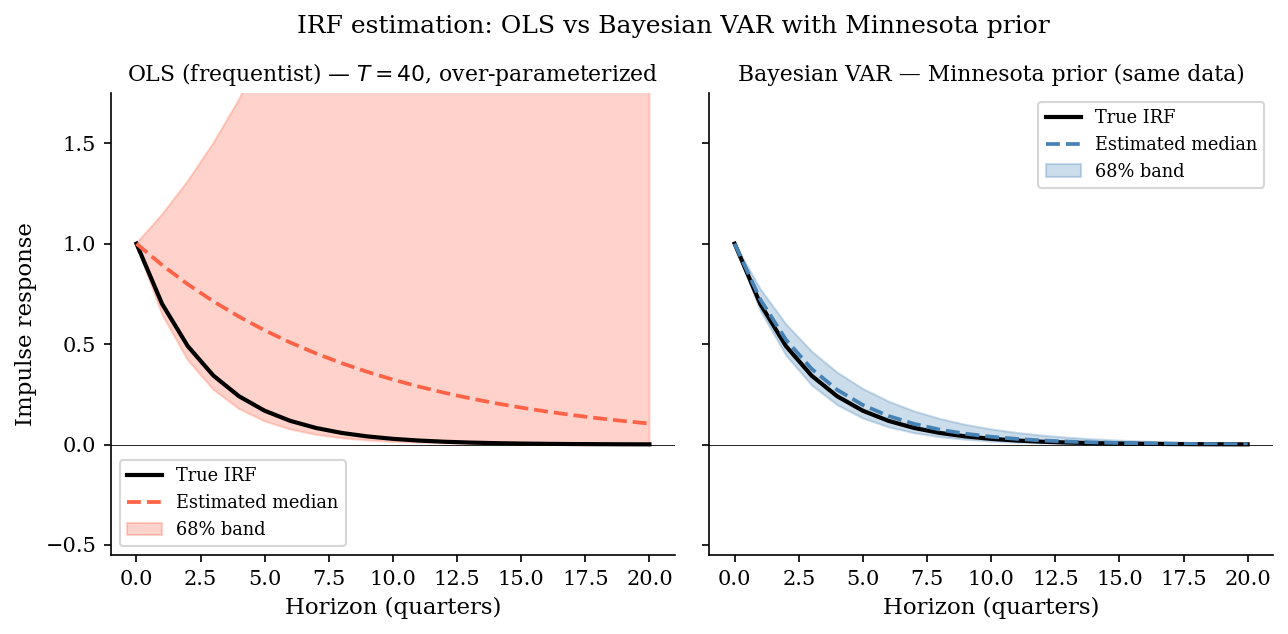
\includegraphics[width=0.97\textwidth]{image/minnesota_irf.png}
\end{center}
\vspace{-0.3cm}
\footnotesize\centering
Same short dataset ($T=40$, $k=6$ variables).\\

\textbf{Left:} OLS bands are wide and can include explosive IRFs.\\

\textbf{Right:} Minnesota prior shrinks toward the random walk $\Rightarrow$ tighter, better-centred bands.\\

Black line = true IRF (AR(1) with $\phi=0.70$).
\end{frame}


%======================================================
\begin{frame}{Prior 2 - Normal-Wishart Prior}
%======================================================
\footnotesize

\textbf{A fully conjugate prior} - treats $\Sigma$ as unknown (unlike the original Minnesota).

\medskip
\textbf{Prior:}
\[
\Sigma \sim \mathcal{IW}(\underline{S},\, \underline{\nu})
\qquad\text{(Inverse-Wishart)}
\]
\[
\text{vec}(B) \mid \Sigma \sim \mathcal{N}\!\left(\text{vec}(\underline{B}),\; \Sigma \otimes \underline{V}\right)
\qquad\text{(Normal conditional on } \Sigma\text{)}
\]

\medskip
\textbf{Posterior:} because of conjugacy, the posterior is also Normal-Wishart:
\[
\Sigma \mid Y \sim \mathcal{IW}(\overline{S},\, \overline{\nu}), \qquad
\text{vec}(B) \mid \Sigma, Y \sim \mathcal{N}(\text{vec}(\overline{B}),\, \Sigma \otimes \overline{V})
\]
with analytical update formulas $(\underline{B}, \underline{V}, \underline{S}, \underline{\nu}) \to (\overline{B}, \overline{V}, \overline{S}, \overline{\nu})$.

\medskip
\textbf{Advantages:}
\begin{itemize}
  \item \textbf{No MCMC needed.} Posterior is available in closed form $\Rightarrow$ \textbf{extremely fast}.
  \item Posterior predictive is a matrix-$t$ distribution (also analytical).
  \item Marginal likelihood is analytical $\Rightarrow$ easy model comparison.
\end{itemize}

\textbf{Limitation:} the $\Sigma \otimes \underline{V}$ structure forces the same $\underline{V}$ across equations.
Cross-equation dependence in the prior cannot be freely specified.

\textbf{Use case:} when analytical tractability and computational speed matter. Baseline in many software packages (e.g.\ \texttt{BEAR6}, \texttt{BVARs.jl}).

\end{frame}


%======================================================
\begin{frame}{Prior 3 - Independent Normal-Wishart Prior}
%======================================================
\footnotesize

\textbf{Motivation:} relax the Kronecker structure $\Sigma \otimes \underline{V}$ of the Normal-Wishart.

\medskip
\textbf{Prior:}
\[
B \mid \Sigma \sim \mathcal{MN}(\underline{B},\, \underline{V}_B,\, \underline{V}_\Sigma),
\qquad
\Sigma \sim \mathcal{IW}(\underline{S},\, \underline{\nu})
\]
but now $\underline{V}_B$ (prior precision on $B$) and $\underline{V}_\Sigma$ (prior on $\Sigma$) are \textbf{independent} across equations.

\medskip
\textbf{In practice:} each equation $i$ gets its own prior variance $V_{B,i}$ on its coefficient vector.
Cross-equation dependence in the prior is removed.

\medskip
\textbf{Posterior:} no longer fully analytical. Requires \textbf{Gibbs sampling} (alternating draws of $B \mid \Sigma, Y$ and $\Sigma \mid B, Y$), but both full conditionals are standard distributions $\Rightarrow$ easy and fast Gibbs.

\medskip
\textbf{Advantages:}
\begin{itemize}
  \item Allows different degrees of shrinkage \textbf{\emph{per equation}} (e.g.\ investment equation is less predictable than consumption $\Rightarrow$ looser prior for that equation).
  \item More flexible than Normal-Wishart while remaining computationally cheap.
\end{itemize}

\textbf{Use case:} when equations are believed to be \textbf{largely independent} in their dynamics
(e.g.\ different sectors of the economy or equations with very different variable sets).

\end{frame}


%======================================================
\begin{frame}{Prior 4 - Normal-Diffuse Prior}
%======================================================
\footnotesize

\textbf{Motivation:} what if we want to shrink the coefficients $B$ but have \textbf{no strong view on $\Sigma$}?

\medskip
\textbf{Prior:}
\[
\text{vec}(B) \sim \mathcal{N}(\text{vec}(\underline{B}),\, \underline{V}_B)
\qquad\text{(informative - Minnesota-type shrinkage)}
\]
\[
p(\Sigma) \propto |\Sigma|^{-(k+1)/2}
\qquad\text{(Jeffreys / diffuse - let data determine $\Sigma$)}
\]

\medskip
\textbf{Posterior:} not fully conjugate. Requires Gibbs:
\begin{itemize}
  \item $B \mid \Sigma, Y \sim \mathcal{N}(\overline{B}, \overline{V}_B)$ - analytical.
  \item $\Sigma \mid B, Y \sim \mathcal{IW}(\hat{E}'\hat{E},\, T-kp)$ where $\hat{E} = Y - XB$ - analytical.
\end{itemize}

\medskip
\textbf{Interpretation:}
\begin{itemize}
  \item Coefficient shrinkage \textbf{without} restricting the error covariance structure.
  \item Useful when the researcher has strong priors on dynamics (e.g.\ from theory) but wants the
        residual covariances to be entirely data-driven.
\end{itemize}

\textbf{Use case:} SFC or structural models where theory pins down some behavioral equations
but the error structure is left unrestricted.

\end{frame}


%======================================================
\section{Time-Varying Bayesian VARs}
%======================================================

%======================================================
\begin{frame}{From Constant to Time-Varying Parameters}
%======================================================
\small

\textbf{All VARs so far assumed:} coefficients $B$ (and $\Sigma$) are \textbf{fixed over time}.

\medskip
\textbf{But in macro:}
\begin{itemize}
  \item The Great Moderation (mid-1980s): volatility halved. Was it a change in $B$ or a change in shocks?
  \item ZLB (2008-2015): monetary transmission changed.
  \item Financial globalization: cross-country spillovers strengthened over time. Etc etc...
\end{itemize}

\pause
\medskip
\textbf{Two dimensions of time variation:}
\begin{enumerate}
  \item \textbf{Time-varying parameters (TVP):} the VAR coefficients $B_t$ change over time  $\Rightarrow$ captures \textbf{gradual structural change} (we studied it).
  \item \textbf{Stochastic volatility (SV):} the error covariance $\Sigma_t$ changes over time
        $\Rightarrow$ captures \textbf{heteroskedasticity} (crisis = larger shocks).
\end{enumerate}

\medskip
Both can be combined. Estimating fixed-parameter VARs in the presence of either naturally leads to \textbf{biased coefficients and wrong inference.}

\end{frame}


%======================================================
\begin{frame}{Time-Varying VAR (TVP-VAR): State-Space Formulation}
%======================================================
\footnotesize

\textbf{TVP-VAR (Cogley \& Sargent, 2001, 2005; Primiceri, 2005):}

\medskip
\textbf{Observation equation (VAR):}
\[
y_t = X_t' \beta_t + u_t, \qquad u_t \sim \mathcal{N}(0, \Sigma_t)
\]

\textbf{State equation (random walk for parameters):}
\[
\beta_t = \beta_{t-1} + \eta_t, \qquad \eta_t \sim \mathcal{N}(0, Q)
\]

\begin{itemize}
  \item $\beta_t$: time-varying VAR coefficients. Follow a \textbf{random walk} - gradual drift, not abrupt breaks like TVAR. $Q$ controls \textbf{how fast} coefficients can move.
  \item $\Sigma_t$: time-varying error covariance - stochastic volatility component.
  \item The full model is a \textbf{state-space system}: estimated by the \textbf{Kalman filter + smoother} (for linear Gaussian case) or \textbf{particle filter} (nonlinear).
\end{itemize}

\medskip
\textbf{Bayesian estimation:}
\begin{itemize}
  \item Prior on $Q$ (e.g.\ Inverse-Wishart) controls how much $\beta_t$ is allowed to move.
  \item Gibbs sampler: draw $\{\beta_t\}_{t=1}^T$ jointly using the \textbf{Carter-Kohn} forward-backward algorithm, then draw $Q$, $\Sigma_t$, etc.\ conditionally.
\end{itemize}

\end{frame}


%======================================================
\begin{frame}{TVP-VAR: Illustration}
%======================================================
\begin{center}
  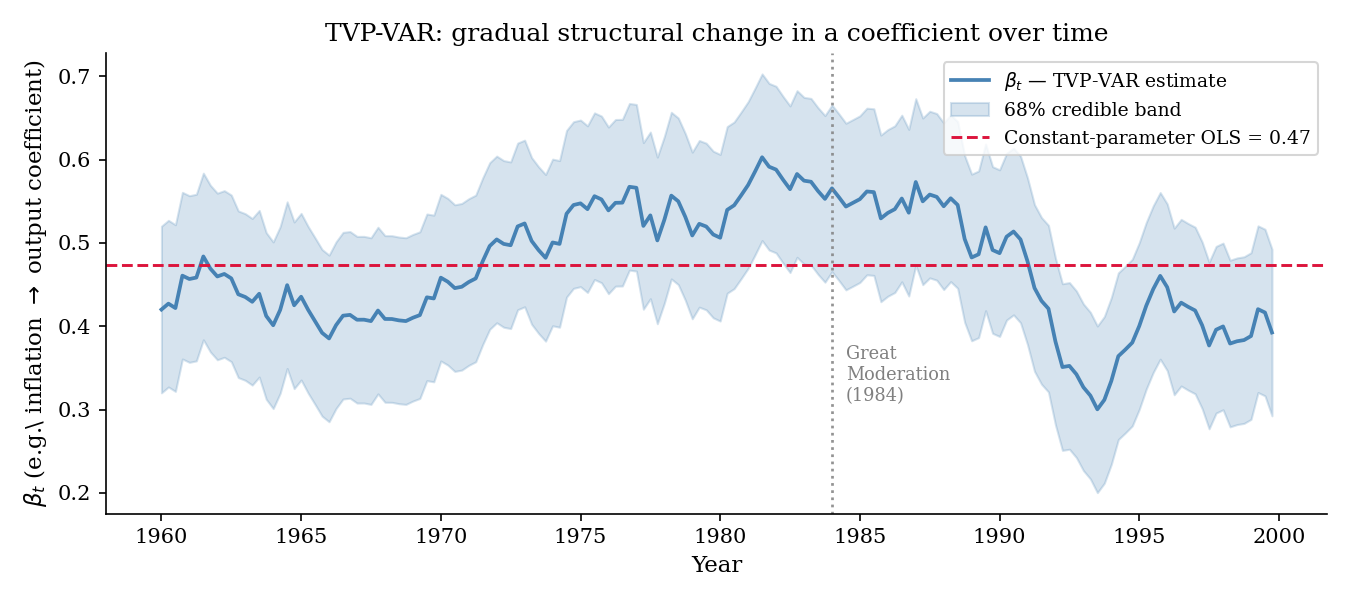
\includegraphics[width=0.94\textwidth]{image/tvp_coefficients.png}
\end{center}
\vspace{-0.3cm}
\footnotesize\centering
TVP-VAR: coefficient $\beta_t$ drifts gradually (random-walk state equation, $Q$ small). The constant-parameter OLS estimate (dashed red) badly summarises a time-varying relationship, here an inflation-output link that weakens after the Great Moderation (1984).
\end{frame}


%======================================================
\begin{frame}{Stochastic Volatility (The Core Idea)}
%======================================================
\footnotesize

\textbf{(Trivial) observation:} macro time series have \textbf{non-constant volatility}.
Crisis periods: large $\sigma_t$. Tranquil periods: small $\sigma_t$.

\medskip
\textbf{Standard SV model} (for a univariate residual $u_t$):
\[
u_t = e^{h_t/2}\, \varepsilon_t, \qquad \varepsilon_t \sim \mathcal{N}(0,1)
\]
\[
h_t = \mu_h + \phi_h (h_{t-1} - \mu_h) + \sigma_h\, w_t, \qquad w_t \sim \mathcal{N}(0,1)
\]
\begin{itemize}
  \item $h_t$: log-variance, evolves as an \textbf{AR(1)}.
  \item $\phi_h \in (-1,1)$: persistence of volatility (typically $\approx 0.95$ in macro - very persistent).
  \item $\sigma_h$: volatility of volatility.
\end{itemize}

\medskip
\textbf{Why log-variance and not variance directly?}
\begin{itemize}
  \item $e^{h_t} > 0$ always: no risk of negative variances.
  \item Log-normal is more tractable than truncated distributions.
\end{itemize}

\medskip
\textbf{In practice:} the SV model is \textbf{non-Gaussian} and \textbf{non-linear} in $h_t$
$\Rightarrow$ requires MCMC (Kim-Shephard-Chib (1998) auxiliary mixture sampler, or particle MCMC).

\end{frame}


%======================================================
\begin{frame}{Stochastic Volatility: Illustration}
%======================================================
\begin{center}
  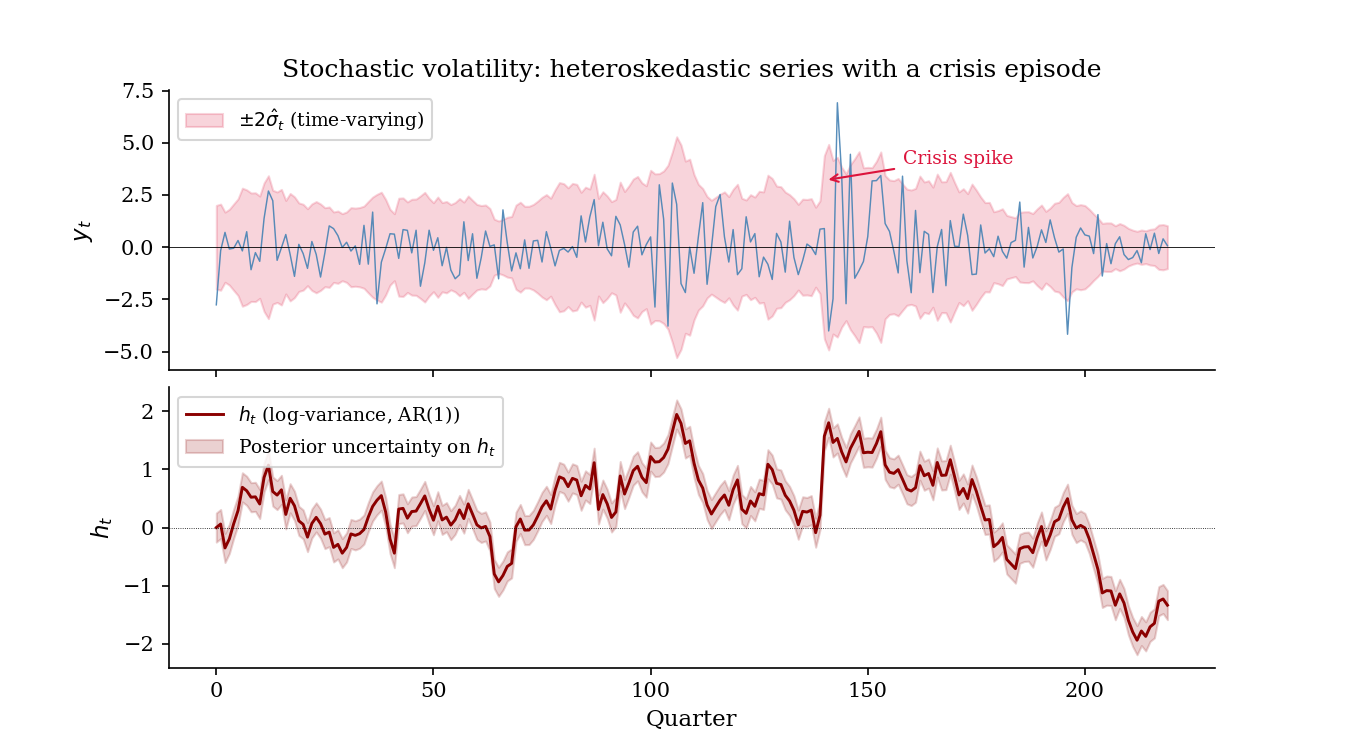
\includegraphics[width=0.94\textwidth]{image/stochastic_volatility.png}
\end{center}
\vspace{-0.3cm}
\footnotesize\centering
\textbf{Top:} simulated series $y_t=e^{h_t/2}\varepsilon_t$; red shading = $\pm 2\hat\sigma_t$ (time-varying).\\

\textbf{Bottom:} log-variance $h_t$ following an AR(1) - persistent, mean-reverting, with a large crisis shock at $t=140$. A constant-variance model would massively misestimate uncertainty throughout.
\end{frame}


%======================================================
\begin{frame}{A Taxonomy of Time-Varying BVARs (in \texttt{BEAR6})}
%======================================================
\scriptsize

\renewcommand{\arraystretch}{1.35}
\begin{tabular}{p{2.6cm} p{3.2cm} p{4.8cm}}
\toprule
\textbf{Model} & \textbf{What varies?} & \textbf{Use case / key feature} \\
\midrule
\textbf{TVP-VAR} \newline(BetaTV) &
  Coefficients $\beta_t$ only \newline(random walk) &
  Gradual structural change in dynamics; constant volatility. \\

\textbf{TVP-VAR-SV} \newline(GeneralTV) &
  Coefficients $\beta_t$ \textbf{and} covariance $\Sigma_t$ &
  Most flexible: both dynamics and volatility evolve. Standard benchmark for policy analysis (Primiceri, 2005). \\

\textbf{Cogley-Sargent SV} \newline(CogleySargentSV) &
  $\Sigma_t$ only (constant $\beta$) &
  Focus on evolving volatility; simpler than full TVP. Good starting point. \\

\textbf{Carriero SV} \newline(CarrieroSV) &
  $\Sigma_t$ via factor structure &
  Large VARs with SV: decomposes $\Sigma_t = A^{-1} H_t A^{-\prime}$ for scalability. \\

\textbf{CCMM SV} \newline(CCMMSV) &
  $h_t$ follows a random walk &
  Persistent, smooth volatility changes (Chan, Koop, Poirier \& Tobias). \\

\textbf{CCMM SV + Outliers} \newline(CCMMSVO) &
  SV + occasional large deviations &
  Robust to \textbf{outliers}: adds a mixture component for rare but extreme observations. \\

\textbf{CCMM SV + Jumps} \newline(CCMMSVOT) &
  SV + jumps in volatility &
  Both smooth drift and \textbf{sudden jumps} in volatility (e.g.\ Lehman, COVID). \\

\textbf{Large Shock SV} \newline(LargeShockSV) &
  $\Sigma_t$ designed for crisis periods &
  Specifically handles samples with \textbf{unusually large innovations} (2008, 2020). \\

\textbf{Random Inertia SV} \newline(RandomInertiaSV) &
  Time-varying \textbf{persistence} $\phi_t$ &
  Shock persistence itself evolves - captures shifts in propagation mechanism. \\
\bottomrule
\end{tabular}

\end{frame}


%======================================================
\begin{frame}{How to Choose Among These Models?}
%======================================================
\footnotesize

\textbf{General principles:}

\begin{enumerate}
  \item \textbf{Start simple.} Constant-parameter Bayesian VAR with Minnesota prior is already much better
        than OLS. Add time-variation only if the data calls for it.

  \item \textbf{Visualize volatility first.} Plot squared residuals of a constant-$B$ VAR.
        If volatility is clearly non-stationary $\Rightarrow$ add SV. If stable $\Rightarrow$ no need.

  \item \textbf{Test for parameter instability.} Structural break tests (Chow, Bai-Perron).
        Strong breaks $\Rightarrow$ TVP or regime-switching. Gradual drift $\Rightarrow$ random walk TVP.

  \item \textbf{Model comparison:}\textbf{ marginal likelihood} (Bayes factor) or
        \textbf{out-of-sample forecast evaluation} (DIC, WAIC, rolling MSFE, backtesting).
        Overly complex models can over-fit even in a Bayesian framework if the prior is not tight enough.

  \item \textbf{Interpretability.} A TVP-SV model with 8 variables produces 8 time-varying IRFs
        for each shock, changing every quarter. Hard to interpret,n only use if the research question requires it (e.g.\ ``Did monetary transmission change post-2008?'').
\end{enumerate}

\end{frame}


%======================================================
\section{Practical Implementation}
%======================================================

%======================================================
\begin{frame}{Bayesian VAR in Practice - Workflow}
%======================================================
\small

\begin{enumerate}
  \item \textbf{Choose variables and transformation.}
        Same as frequentist: stationarity, $I(1)/I(0)$, cointegration.
        A BVAR in levels is possible (Sims-Zha recommendation: include levels if unit roots present,
        the Minnesota prior provides implicit regularization).

  \item \textbf{Choose prior:}
  \begin{itemize}
    \item Homogeneous variables (similar scales, same sector) $\Rightarrow$ Minnesota / Normal-Wishart.
    \item Heterogeneous equations $\Rightarrow$ Independent Normal-Wishart.
    \item Strong volatility variation in the sample $\Rightarrow$ add SV.
    \item Known structural changes $\Rightarrow$ TVP.
  \end{itemize}

  \item \textbf{Set hyperparameters} $(\lambda_1, \lambda_2, \lambda_3)$.
  Optimal: maximize marginal likelihood (``hierarchical Bayes'' - data chooses tightness).

  \item \textbf{Estimate:} analytical posterior (Normal-Wishart) or Gibbs sampler.
        Check convergence (trace plots, $\hat R$).

  \item \textbf{Inference:} posterior draws $\Rightarrow$ IRFs with credible bands, FEVD,
        forecast distributions.

  \item \textbf{Validate:} pseudo out-of-sample forecasting, residual diagnostics.
\end{enumerate}

\end{frame}


%======================================================
\begin{frame}{Bayesian VAR - Forecasting in Practice}
%======================================================
\footnotesize

\textbf{The posterior predictive distribution} integrates over parameter uncertainty:
\[
p(y_{T+1}, \dots, y_{T+H} \mid Y) = \int p(y_{T+1:T+H} \mid B, \Sigma)\, p(B, \Sigma \mid Y)\, dB\, d\Sigma
\]

\textbf{Algorithm:}
\begin{enumerate}
  \item For each posterior draw $(B^{(s)}, \Sigma^{(s)})$:
  \begin{enumerate}
  \footnotesize
    \item Simulate shocks $u_{T+h}^{(s)} \sim \mathcal{N}(0, \Sigma^{(s)})$, $h=1,\dots,H$.
    \item Compute $y_{T+h}^{(s)} = X_{T+h}^{(s)\prime} B^{(s)} + u_{T+h}^{(s)}$ recursively.
  \end{enumerate}
  \item The cloud $\{y_{T+h}^{(s)}\}_{s=1}^S$ \textbf{is} the forecast distribution.
        Report median + 68\% and 90\% credible intervals.
\end{enumerate}

\medskip
\textbf{Empirical performance:}
\begin{itemize}
  \item Banbura, Giannone \& Reichlin (2010): large BVARs with Minnesota prior
        \textbf{outperform small VARs and univariate benchmarks} at all horizons.
  \item Giannone, Lenza \& Primiceri (2015): optimal hyperparameters selected by marginal likelihood.
        Forecasts competitive with factor models (DFMs).
  \item During COVID (2020): models with SV and outlier robustness (CCMMSVO, LargeShockSV)
        clearly dominated standard BVARs.
\end{itemize}

\end{frame}


%======================================================
\begin{frame}{Bayesian VAR - Forecast Fan Chart}
%======================================================
\begin{center}
  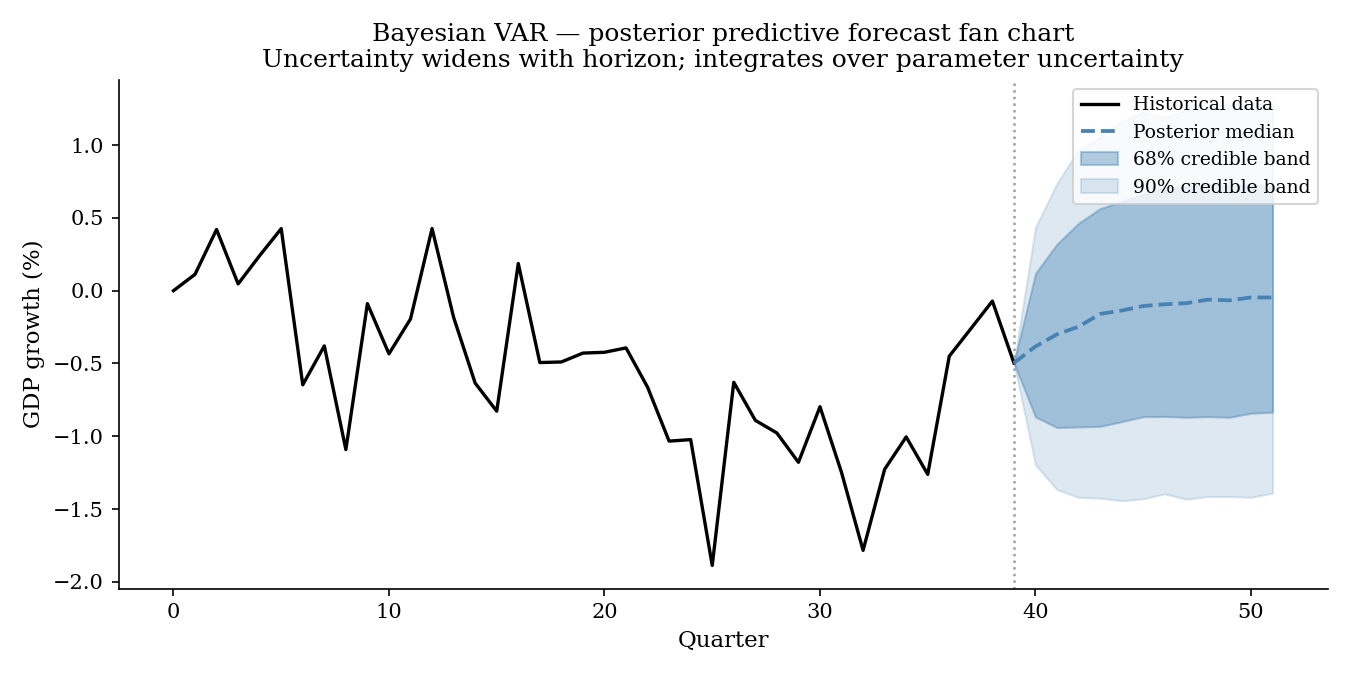
\includegraphics[width=0.94\textwidth]{image/forecast_fan.png}
\end{center}
\vspace{-0.3cm}
\footnotesize\centering
Posterior predictive fan chart: the 68\% and 90\% credible bands widen naturally with the horizon, reflecting both shock uncertainty and \textbf{parameter uncertainty} (each draw of $(B^{(s)},\Sigma^{(s)})$ gives a different propagation path). A plug-in forecast using only the posterior mean of $\phi$ would \emph{under}estimate uncertainty.
\end{frame}


%======================================================
\begin{frame}{IRFs from Bayesian VARs}
%======================================================
\footnotesize

\textbf{Same identification strategies as frequentist SVARs:}
Cholesky, short-run, long-run, sign, heteroskedasticity restrictions, spectral max-share, proxy-VAR... applied to each posterior draw.

\medskip
\textbf{Algorithm (Cholesky example):}
\begin{enumerate}
  \item Draw $(B^{(s)}, \Sigma^{(s)})$ from posterior.
  \item Compute Cholesky: $\Sigma^{(s)} = P^{(s)} P^{(s)\prime}$.
  \item Compute reduced-form MA matrices $\Phi_h^{(s)}$ from $B^{(s)}$.
  \item Structural IRF$_h^{(s)} = \Phi_h^{(s)} P^{(s)}$.
\end{enumerate}
Repeat for $s = 1, \dots, S$ $\Rightarrow$ \textbf{posterior distribution of IRFs}.

\medskip
\textbf{Credible bands vs. frequentist confidence bands:}
\begin{itemize}
  \item Frequentist: ``if we repeated the data-generating process infinitely, 68\% of these bands would contain the true IRF.''
  \item Bayesian: ``given the data and the prior, the IRF lies in this region with probability 68\%.''
  \item In practice with $T=120$: Bayesian bands are \textbf{narrower and better calibrated}
        (no delta-method approximation, no asymptotic normality assumed).
\end{itemize}

\end{frame}


%======================================================
\begin{frame}{Summary}
%======================================================
\footnotesize

\begin{block}{What Bayesian estimation brings to macro}
\begin{enumerate}
  \item \textbf{Regularization:} priors shrink parameters toward economically sensible benchmarks.
        Solves the over-parameterization problem of VARs.
        \item \textbf{Use of theoretical priors and already-existing empirics.}
  \item \textbf{Full uncertainty quantification:} posterior distributions, credible bands,
        posterior predictive (not just point estimates $+$ asymptotic SEs).
  \item \textbf{Time variation if needed} (state-space $+$ Gibbs sampler for
        TVP and SV models otherwise intractable).
  \item \textbf{Model comparison:} marginal likelihood selects models without $p$-value hacking.
\end{enumerate}
\end{block}


\end{frame}


\end{document}
